\chapter{Fundamentação Teórica}
\label{cap:fundamentacao-teorica}

Este capítulo apresenta os conceitos fundamentais e o panorama tecnológico que sustentam o desenvolvimento deste estudo. Inicialmente, a Seção~\ref{sec:llms_e_alucinacoes} aborda os grandes modelos de linguagem (LLMs) e o impacto das alucinações semânticas no contexto educacional, motivando a discussão, na Seção~\ref{sec:rag_tradicional}, sobre o funcionamento da arquitetura de Geração Aumentada por Recuperação (RAG) tradicional e suas limitações estruturais diante de documentos didáticos complexos. Para superar tais desafios, a Seção~\ref{sec:rag_multimodal} introduz o paradigma RAG Multimodal (MRAG), destacando o papel dos modelos de linguagem e visão (VLMs) e a importância da granularidade fina no controle do ruído contextual. A viabilização dessa granularidade é explorada na Seção~\ref{sec:segmentacao_layout}, que analisa técnicas de Análise de Layout de Documentos (DLA) para o isolamento de componentes estruturais em arquivos PDF. Por fim, a Seção~\ref{sec:engenharia_contexto} discute a engenharia de contexto como um mecanismo essencial para a mitigação proativa de alucinações e a garantia da rastreabilidade das evidências retornadas ao usuário.

\section{Grandes modelos de linguagem e alucinações no ensino}
\label{sec:llms_e_alucinacoes}

A compreensão, interpretação e geração da linguagem humana por computadores constituem alguns dos desafios mais antigos e centrais da Ciência da Computação, especialmente no campo do Processamento de Linguagem Natural (PLN) \citeb{jurafsky2024speech}. Nos últimos anos, essa área passou por avanços significativos com o surgimento dos Grandes Modelos de Linguagem, ou \textit{Large Language Models} (LLMs), que formam a base tecnológica de muitos sistemas conversacionais e geradores de texto atuais \citeb{zhao2026survey}. Esse avanço foi impulsionado pela arquitetura \textit{Transformer}, introduzida por \citeonline{vaswani2017attention}, baseada no mecanismo de autoatenção (\textit{self-attention}), que permite ao modelo considerar simultaneamente diferentes partes de um texto. Diferentemente de abordagens sequenciais tradicionais, essa característica favorece a identificação de relações contextuais entre termos, frases e trechos ao longo de um documento.

Por trás da aparente inteligência dessas ferramentas, o funcionamento básico de um LLM baseia-se em processos probabilísticos. Diante de uma pergunta ou comando, o modelo utiliza mecanismos de autoatenção não para consultar uma base de dados estática de informações verificadas, mas para analisar o contexto fornecido na entrada e estimar, token por token, qual é a continuação mais provável para aquela sequência \citeb{tunstall2022natural}. Como esse processo se apoia em padrões estatísticos aprendidos durante o treinamento, o sistema tende a priorizar a construção de respostas que pareçam naturais e coerentes para quem lê, mesmo que o modelo não possua, por si só, um mecanismo nativo de verificação factual das informações geradas \citeb{wolfram2023chatgpt}.

Essa natureza estatística contribui para uma limitação estrutural relevante dos LLMs, conhecida como alucinação semântica. Esse fenômeno ocorre quando a inteligência artificial gera respostas linguisticamente coerentes, mas que apresentam informações falsas, imprecisas ou não fundamentadas. Na literatura técnica, essas falhas costumam ser divididas em duas categorias: alucinações intrínsecas, quando o modelo contradiz ou ignora informações fornecidas pelo próprio usuário no comando; e alucinações extrínsecas, quando o sistema introduz fatos, nomes ou regras que não são sustentados pelas fontes disponíveis \citeb{Ji_2023}. Esse comportamento pode estar relacionado a inconsistências e vieses presentes nos dados de treinamento, bem como à tendência dos modelos de produzir continuações textuais plausíveis mesmo quando não possuem evidências suficientes para sustentar a resposta \citeb{alansari2026large}.

No ambiente de ensino, essa vulnerabilidade técnica assume implicações pedagógicas relevantes, uma vez que o uso de LLMs como tutores individualizados pode estabelecer uma relação de confiança entre o estudante e a ferramenta \citeb{kasneci2023chatgpt}. Conforme alertam os autores, por estar em processo de aquisição e consolidação de conhecimento, o aluno nem sempre possui o repertório necessário para identificar alucinações sutis, especialmente quando elas aparecem em respostas formuladas com coerência, fluidez e aparente autoridade. Esse cenário, conforme corroborado por \citeonline{holmes2023guidance}, pode induzir o estudante ao erro de maneira pouco perceptível, favorecendo a consolidação de equívocos conceituais e comprometendo a qualidade do processo de aprendizagem.

\section{Geração aumentada por recuperação tradicional e suas limitações}
\label{sec:rag_tradicional}

Como forma de mitigar as alucinações semânticas e ampliar a base de conhecimento dos LLMs sem a necessidade de novos processos custosos de treinamento, a comunidade de inteligência artificial desenvolveu o conceito de Geração Aumentada por Recuperação (RAG) \citeb{NEURIPS2020_6b493230}. Em sua abordagem tradicional, também conhecida como RAG linear ou ingênua (\textit{Naive RAG}), esse paradigma é descrito por \citeonline{gao2023retrieval} como a integração entre um mecanismo de busca e um modelo gerador. Nesse fluxo, os documentos didáticos em PDF são inicialmente convertidos em conteúdo textual e segmentados em blocos menores, por meio da técnica de \textit{chunking}.

A dinâmica de consulta desse ecossistema ocorre em tempo de execução, a partir da interação do usuário. Nesse momento, a pergunta submetida é processada pelo mesmo modelo de codificação utilizado na etapa de indexação, gerando um vetor de busca semanticamente equivalente. Conforme detalhado por \citeonline{tunstall2022natural}, o sistema executa então uma busca vetorial na base de dados por meio de cálculos de proximidade, identificando os blocos de conteúdo cujo contexto apresenta maior alinhamento semântico com a dúvida enviada. Os fragmentos recuperados são inseridos no \textit{prompt} de entrada do LLM, servindo como base de conhecimento complementar. Dessa forma, de acordo com o paradigma proposto por \citeonline{NEURIPS2020_6b493230}, o modelo gerador passa a construir a resposta com apoio em informações previamente recuperadas de fontes verificáveis, em vez de depender exclusivamente dos padrões aprendidos durante seu treinamento.
 
Apesar do bom desempenho dessa abordagem em textos corridos e lineares, o RAG tradicional apresenta limitações estruturais quando aplicado a documentos com layout complexo, como livros didáticos e materiais de estudo em formato PDF. Um dos principais desafios está na perda ou simplificação de elementos não textuais, uma vez que tabelas, gráficos, infográficos e diagramas explicativos nem sempre são adequadamente preservados por extratores de texto convencionais, limitando o acesso do LLM a informações visuais relevantes para o aprendizado \citeb{faysse2025colpali}. Além disso, a segmentação do documento em blocos de tamanho fixo pode comprometer a ordem lógica da informação, fragmentando hierarquias visuais e comprometendo a qualidade do contexto fornecido ao modelo de linguagem \citeb{gao2023retrieval}.

\subsection{Representação semântica e embeddings}
\label{subsec:embeddings}

Para que algoritmos de busca processem o conhecimento externo matematicamente, o texto extraído dos documentos precisa ser convertido em vetores numéricos de alta dimensão, conhecidos como \textit{embeddings}. Esse processo evoluiu de forma significativa com o surgimento do BERT (\textit{Bidirectional Encoder Representations from Transformers}). Baseado na arquitetura \textit{Transformer}, esse modelo de linguagem foi projetado para capturar o contexto bidirecional das palavras em um texto \citeb{devlin2019bert}.

Ao utilizar modelos de vetorização derivados dessa tecnologia, os fragmentos de texto são projetados em um espaço vetorial contínuo. Essa projeção captura o significado semântico do conteúdo e aproxima geometricamente frases com sentidos semelhantes. Como resultado, torna-se possível a transição de uma busca puramente léxica para uma recuperação verdadeiramente semântica \citeb{DBLP:journals/corr/abs-1908-10084}.

No contexto multilíngue, modelos como o BGE-M3, proposto por \citeonline{chen2024bge}, ampliam essa capacidade ao suportar entradas em diferentes idiomas e granularidades textuais, desde sentenças isoladas até parágrafos completos. Sua arquitetura reúne três funcionalidades de recuperação em um único modelo: recuperação densa, baseada em \textit{embeddings} semânticos de alta dimensionalidade; recuperação esparsa, fundamentada em pesos lexicais; e interação de múltiplos vetores, que permite representar um mesmo documento por meio de múltiplos \textit{embeddings}.

Essa combinação torna o BGE-M3 particularmente adequado para sistemas de recuperação que precisam indexar fragmentos semanticamente heterogêneos. Em documentos didáticos segmentados em componentes estruturais distintos, como títulos, parágrafos, legendas e descrições visuais geradas automaticamente, todos esses elementos podem ser projetados em um espaço vetorial comum, permitindo buscas por similaridade semântica de forma uniforme.


\subsection{Similaridade vetorial e recuperação por proximidade}
\label{subsec:similaridade_vetorial}

Uma vez que tanto os componentes do documento quanto a consulta formulada pelo usuário são projetados no mesmo espaço vetorial, o mecanismo de busca atua calculando a distância matemática entre eles. A métrica predominante em arquiteturas RAG é a similaridade de cosseno \citeb{gao2023retrieval}, que avalia o ângulo formado entre dois vetores no espaço multidimensional, ignorando a magnitude absoluta. A Figura~\ref{fig:similaridade_cosseno} ilustra essa relação geométrica, demonstrando como os diferentes ângulos refletem os graus de similaridade.

\begin{figure}[H]
\centering
\begin{minipage}{\textwidth}
\caption{Representação geométrica da métrica de similaridade de cosseno.}
\label{fig:similaridade_cosseno}
\vspace{0.2cm}
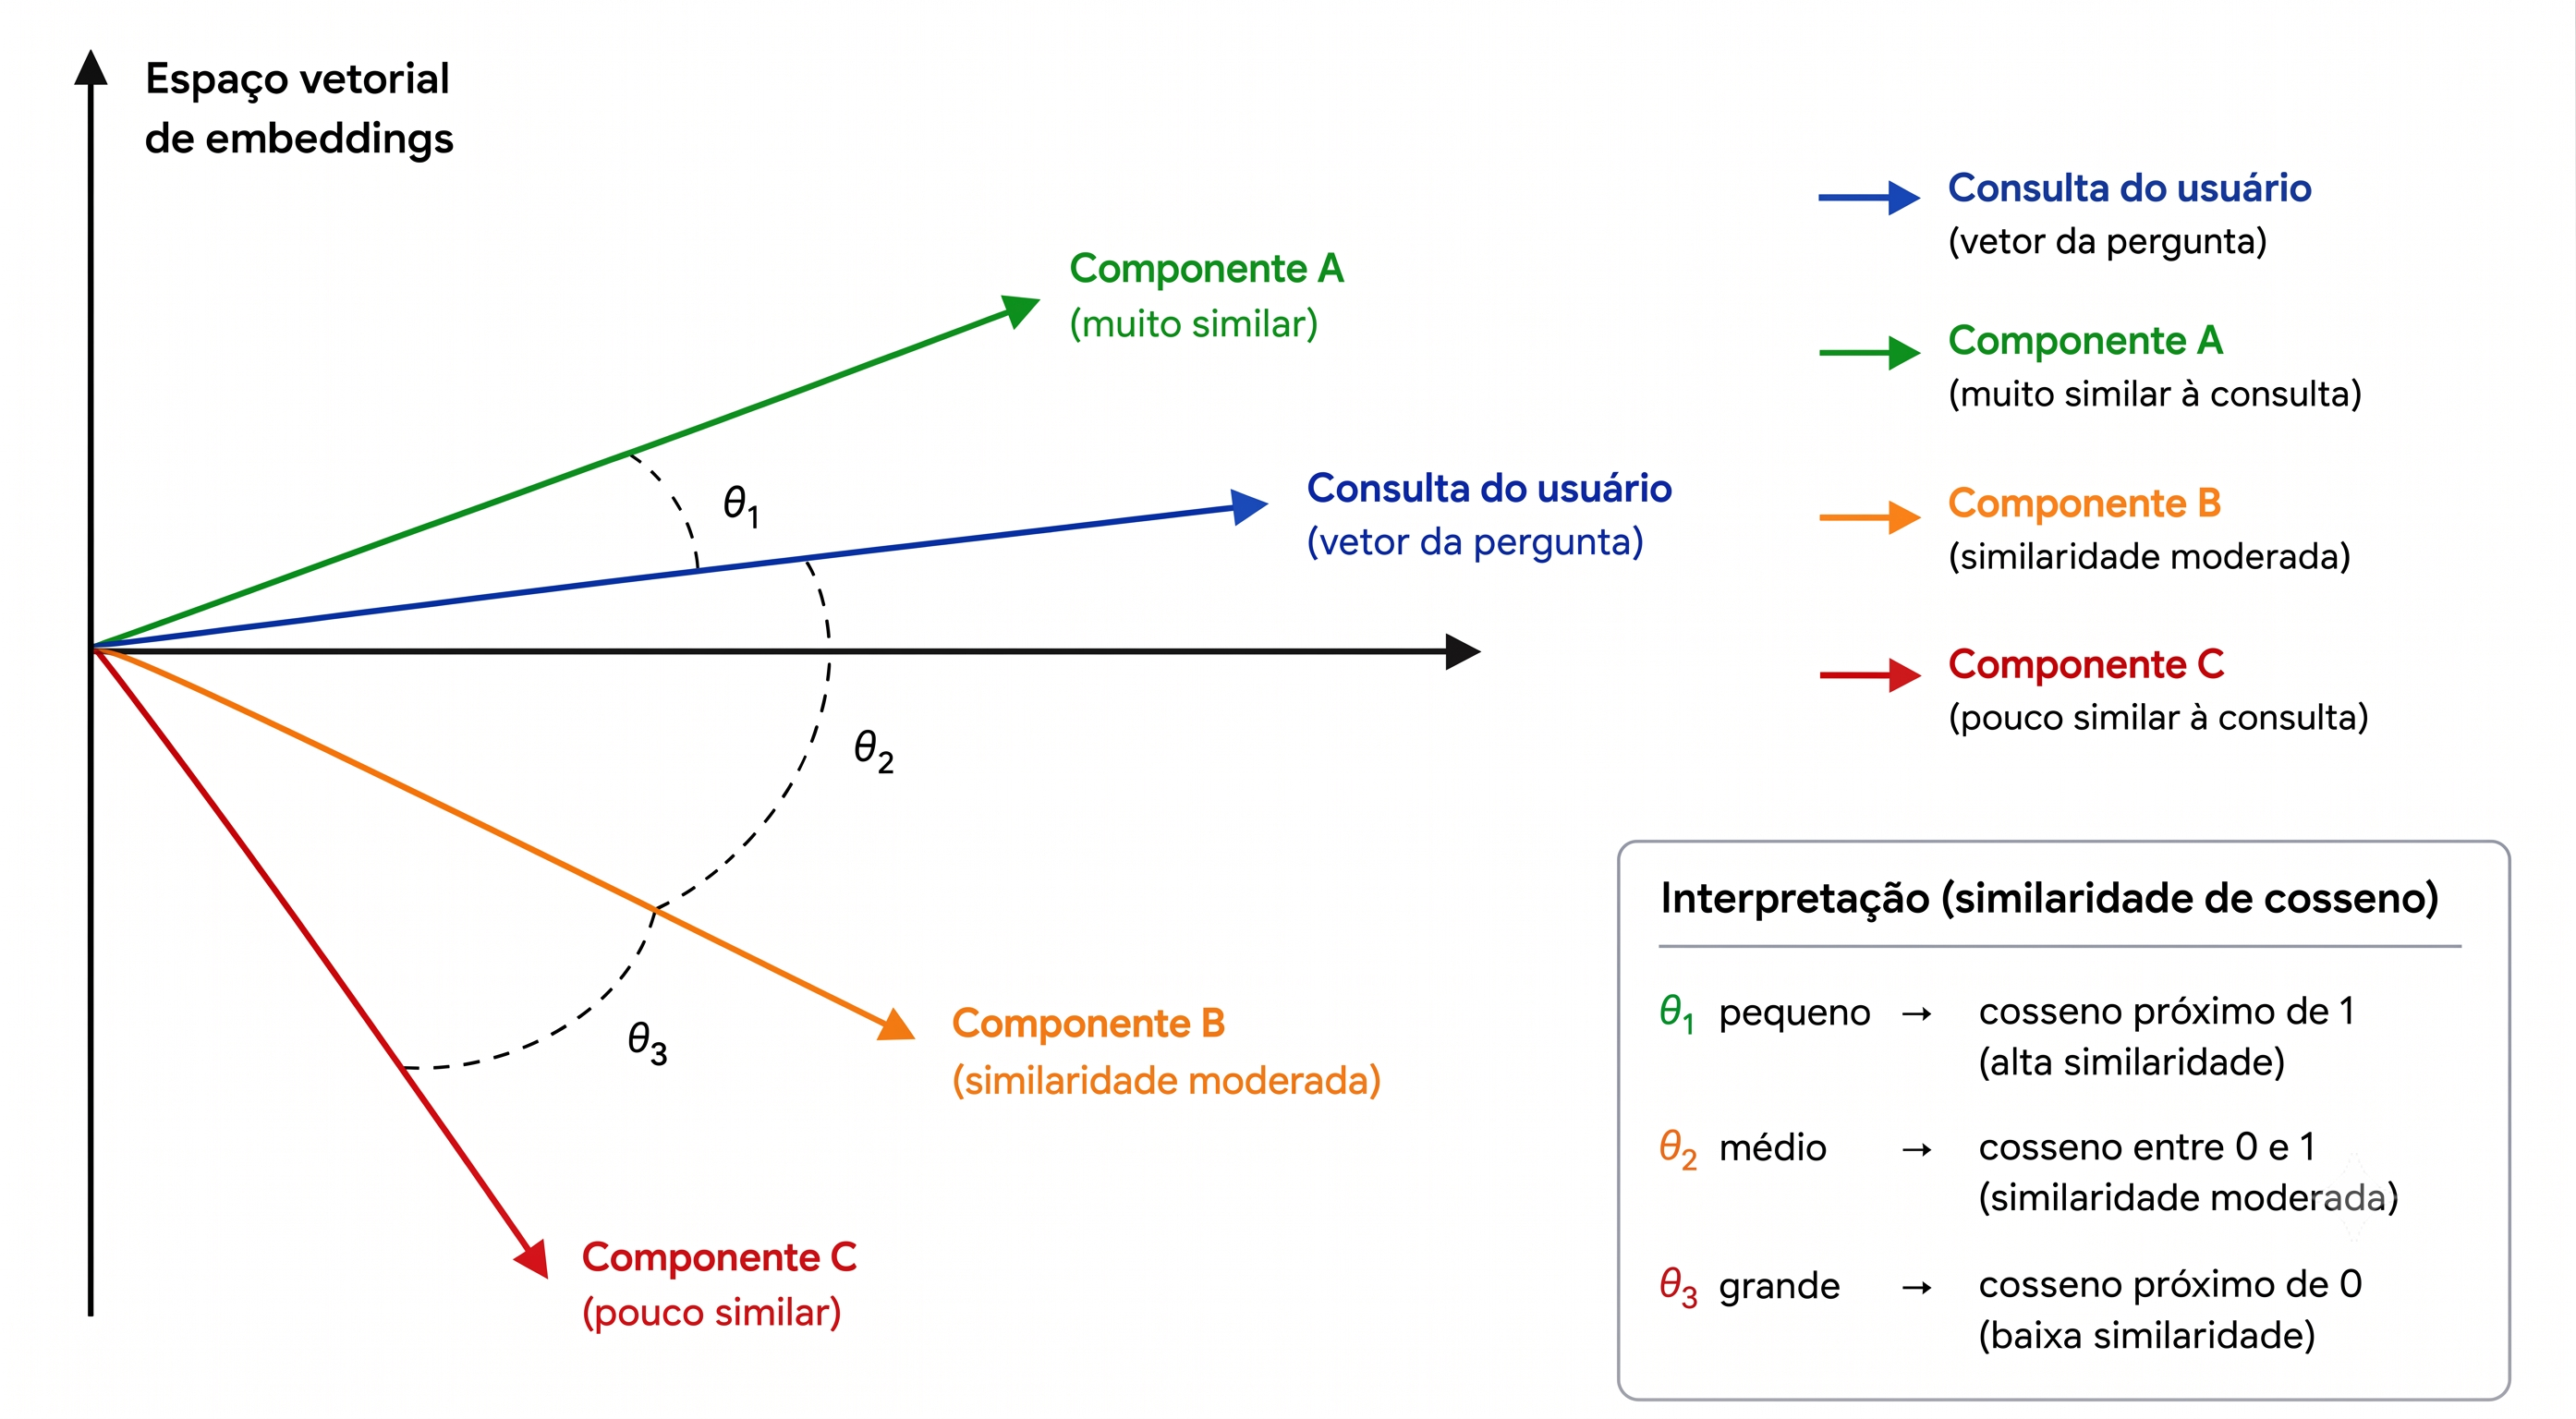
\includegraphics[width=\textwidth]{figuras/similaridade_cosseno}
\vspace{0.1cm}
\\ {\footnotesize Fonte: Elaborado pelo autor.}
\end{minipage}
\end{figure}

No contexto de representações densas, quanto menor o ângulo entre os \textit{embeddings} da consulta e de um componente documental (valor de cosseno próximo a 1), maior é a indicação de proximidade semântica. Esse cálculo rápido e escalável permite que sistemas de recuperação encontrem os blocos de informação que efetivamente respondem à necessidade de informação do usuário, independentemente de variações de vocabulário \citeb{DBLP:journals/corr/abs-1908-10084}.

\subsection{Bancos de dados vetoriais}
\label{subsec:bancos_vetoriais}

Para lidar com a indexação e a recuperação eficiente de milhões de \textit{embeddings} em alta dimensionalidade, sistemas RAG exigem infraestruturas de armazenamento especializadas. Ao contrário dos bancos de dados relacionais tradicionais, que organizam dados em tabelas orientadas a consultas determinísticas, os bancos de dados vetoriais são arquitetados para executar buscas por similaridade aproximada do vizinho mais próximo (\textit{Approximate Nearest Neighbor} -- ANN) \citeb{johnson2019billion}. Adicionalmente, essas ferramentas suportam a estratégia de recuperação híbrida, permitindo anexar metadados estruturados (ou \textit{payloads}) aos vetores \citeb{gao2023retrieval}. No domínio educacional, essa capacidade é indispensável, pois possibilita que a busca vetorial seja filtrada por restrições lógicas, como o identificador do material didático, o número da página ou a classe geométrica do componente visual retornado.

\subsection{Filtragem por metadados em sistemas RAG}
\label{sec:filtragem_metadados}

A busca por similaridade vetorial, descrita na subseção~\ref{subsec:similaridade_vetorial}, opera exclusivamente sobre o espaço de \textit{embeddings}. Dado um vetor de consulta, o sistema retorna os $K$ vizinhos mais próximos sem considerar restrições semânticas associadas aos metadados de cada registro \citeb{karpukhin2020dense}. Essa abordagem é adequada para repositórios homogêneos e de domínio único, mas apresenta limitações quando o banco vetorial reúne componentes provenientes de múltiplos documentos.

Para superar essa limitação, arquiteturas RAG modernas adotam a estratégia de filtragem baseada em metadados (\textit{metadata filtering}), que combina a busca por similaridade vetorial com restrições estruturadas aplicadas aos atributos (ou \textit{payloads}) de cada registro. Nesse modelo, a consulta é processada com base em dois critérios complementares: (i) o ranqueamento por similaridade de cosseno entre o vetor da pergunta e os vetores dos componentes indexados; e (ii) a aplicação de predicados lógicos que restringem o espaço de busca a registros que atendem a condições específicas, como pertencer a um determinado documento, estar localizado em um intervalo de páginas ou possuir uma classe estrutural específica \citeb{gao2023retrieval}.
 
No contexto de aplicações educacionais que lidam com acervos extensos, essa capacidade apresenta-se como uma solução arquitetural necessária. Em cenários nos quais um banco de dados vetorial armazena simultaneamente múltiplos materiais didáticos, a filtragem por metadados permite que a busca seja restrita exclusivamente ao documento ativo na sessão do usuário. Dessa forma, garante-se que apenas os componentes estruturais do material pertinente sejam retornados ao modelo gerador, evitando a contaminação do contexto por informações de outras fontes, independentemente de sua proximidade vetorial.
 

\section{Geração aumentada por recuperação multimodal e modelos de visão}
\label{sec:rag_multimodal}

Para superar parte das limitações do RAG tradicional na interpretação de layouts complexos, a área de inteligência artificial avançou em direção à Geração Aumentada por Recuperação Multimodal (MRAG) \citeb{mei2025survey}. A principal contribuição desse paradigma está na capacidade de alinhar diferentes modalidades de dados, como texto e imagem, em um mesmo espaço vetorial. Sob essa perspectiva, o sistema passa a tratar o material didático não apenas como uma sequência linear de texto, mas também a partir de suas representações visuais e estruturais, correlacionando semanticamente uma dúvida textual a elementos como gráficos, tabelas ou diagramas.

\subsection{Modelos de linguagem e visão (VLMs) para recuperação}
\label{subsec:vlms_recuperacao}

A viabilização do MRAG dependeu fundamentalmente do avanço dos modelos de linguagem e visão (\textit{Vision-Language Models} -- VLMs). Conforme discutido por \citeonline{Yin_2024}, esses modelos reduzem a dependência de intermediários estritos, processando diretamente representações visuais. Nesse contexto, a arquitetura \textit{ColPali}, introduzida por \citeonline{faysse2025colpali}, representa um avanço relevante ao aplicar o conceito de interação tardia (\textit{Late Interaction}) à busca documental. Em vez de compactar uma página inteira em um único vetor, o modelo gera múltiplos \textit{embeddings} associados a diferentes \textit{patches} da imagem. Isso permite que o mecanismo preserve informações contidas em tabelas e fórmulas matemáticas sem necessitar de extração textual prévia.

\subsection{VLMs como modelos geradores de descrições visuais}
\label{subsec:vlms_geradores}

No ecossistema multimodal, é fundamental distinguir os VLMs que atuam exclusivamente como codificadores (\textit{encoders} voltados à recuperação) daqueles que operam como geradores instrucionais (\textit{instruction-following}) \citeb{Yin_2024}. Modelos geradores, como a família Qwen-VL \citeb{bai2023qwen}, possuem a capacidade não apenas de mapear imagens, mas de receber um recorte visual acompanhado de um comando \textit{(prompt)} e produzir um raciocínio textual sobre ele. Essa habilidade permite interpretar fluxogramas estruturados, decodificar relações de grandezas em eixos de gráficos e traduzir diagramas lógicos em texto estruturado. Em \textit{pipelines} documentais, a aplicação desses modelos transforma representações puramente visuais em componentes semânticos ricos e diretamente indexáveis.

\subsection{Ruído contextual e granularidade de recuperação}
\label{subsec:ruido_contextual}

Apesar dos avanços no mapeamento multimodal, a escolha da unidade de recuperação, isto é, sua granularidade, influencia diretamente a precisão do sistema. Em implementações que recuperam a imagem ou o texto de páginas inteiras, é comum que o modelo gerador receba uma grande quantidade de informações acessórias, como rodapés, numerações de página e parágrafos relacionados a outros assuntos \citeb{yun2025lilac}. Esse excesso de conteúdo introduz ruído na janela de contexto. Conforme demonstrado por \citeonline{liu2024lost} no estudo que descreve o fenômeno \textit{Lost in the Middle}, LLMs apresentam degradação significativa em suas capacidades de raciocínio e extração de informações quando submetidos a contextos extensos e contendo dados irrelevantes.

Portanto, em vez de depender da página inteira, a adoção de uma granularidade fina, capaz de isolar visual e textualmente apenas o bloco informacional relevante, surge como uma estratégia importante para reduzir a saturação informacional e mitigar alucinações extrínsecas.

\section{Segmentação de layout e processamento de documentos}
\label{sec:segmentacao_layout}

Para viabilizar a transição da recuperação de páginas inteiras para uma granularidade mais fina, a engenharia de dados aplicada a documentos recorre às técnicas de Análise de Layout de Documentos (\textit{Document Layout Analysis} -- DLA). Essa área estuda métodos capazes de identificar a estrutura geométrica e a organização lógica de documentos digitais \citeb{zhong2019publaynet}. Seu principal objetivo é mapear a página em duas dimensões, detectando e delimitando componentes estruturais, como títulos, parágrafos, tabelas e figuras, por meio de caixas delimitadoras (\textit{bounding boxes}). O mapeamento preciso dessas regiões constitui a base metodológica para o isolamento da informação. Entretanto, para que o conteúdo textual presente nesses blocos seja efetivamente indexado pelo sistema, é necessário convertê-lo de uma representação visual para texto digital.

\subsection{Reconhecimento óptico de caracteres (OCR)}
\label{subsec:ocr}

Para realizar essa conversão, a principal tecnologia utilizada é o Reconhecimento Óptico de Caracteres (OCR), responsável por transformar imagens contendo texto, provenientes de documentos digitalizados ou arquivos rasterizados, em sequências de caracteres digitais pesquisáveis \citeb{smith2007overview}. Tradicionalmente, os sistemas de OCR foram projetados para processar páginas de forma global, percorrendo todo o conteúdo em uma ordem predefinida. No entanto, conforme discutido por \citeonline{shen2021layoutparser}, essa abordagem apresenta limitações significativas quando aplicada a documentos complexos.

Em materiais didáticos que contêm múltiplas colunas, equações e tabelas, o processamento da página como um todo pode levar à combinação incorreta de trechos de texto e à perda da ordem natural de leitura. Para superar esse problema, a integração entre OCR e técnicas de DLA torna-se fundamental. Ao utilizar as \textit{bounding boxes} para orientar a extração textual, o OCR passa a operar de forma localizada, processando cada componente geométrico individualmente. Como resultado, a estrutura original do documento é preservada, mantendo a coerência semântica das informações extraídas e evidenciando a complementaridade entre a análise de layout e o reconhecimento de caracteres \citeb{shen2021layoutparser}.

\subsection{Detecção de objetos aplicada a documentos}
\label{subsec:yolo_documentos}

Para viabilizar computacionalmente a segmentação de layout necessária ao OCR localizado, a literatura impulsionou inicialmente o desenvolvimento de modelos multimodais voltados à compreensão integrada de documentos. Abordagens baseadas em \textit{Transformers}, como as arquiteturas da família \textit{LayoutLM} \citebdois{xu2020layoutlm}{huang2022layoutlmv3}, consolidaram-se como importantes referências ao demonstrar que a posição espacial de um elemento fornece informações semânticas relevantes para a interpretação do documento. Contudo, pesquisadores observam que essa precisão costuma estar associada a um elevado custo computacional, uma vez que esses modelos frequentemente dependem da extração prévia de \textit{tokens} textuais. Em cenários de processamento documental em larga escala, essa característica pode representar um desafio de desempenho, motivando a busca por alternativas mais eficientes baseadas em detecção de objetos.

Fundamentadas no paradigma YOLO (\textit{You Only Look Once}) \citeb{redmon2016you}, arquiteturas especializadas para o domínio documental, como o DocLayout-YOLO \citeb{zhao2024doclayout}, adotam uma abordagem centrada exclusivamente em informações visuais. Em vez de depender da análise textual para identificar a estrutura do documento, esses modelos tratam cada página como uma imagem renderizada e realizam a detecção dos componentes estruturais a partir de seus padrões gráficos. Como consequência, a segmentação do layout pode ser realizada sem a necessidade de etapas prévias de extração textual. A combinação entre independência em relação ao conteúdo textual e baixa latência de inferência torna essa família de modelos particularmente adequada para atuar como etapa inicial em \textit{pipelines} de processamento documental, delimitando os blocos estruturais antes de sua submissão às etapas de OCR seletivo e descrição semântica.


\section{Engenharia de contexto em sistemas RAG}
\label{sec:engenharia_contexto}

A etapa final para garantir a precisão informacional em arquiteturas RAG ocorre na fronteira de comunicação com o modelo de linguagem. A Engenharia de Contexto abrange as estratégias algorítmicas e arquiteturais aplicadas na seleção, organização e refinamento das evidências recuperadas antes de sua inserção no \textit{prompt}. Esta seção aborda as abordagens adotadas para otimizar os dados fornecidos à rede neural e define as métricas automatizadas utilizadas para atestar a qualidade desse processo.

\subsection{Estratégias de seleção e refinamento de contexto}
\label{subsec:estrategias_refinamento_contexto}

Estudos recentes demonstram que a forma como as evidências são organizadas no \textit{prompt} influencia diretamente a acurácia das respostas geradas. O \textit{framework} SLEUTH, proposto por \citeonline{liu2025resolving}, evidenciou que o uso de agentes para iterar e refinar pistas visuais e textuais pode mitigar problemas de dispersão em documentos extensos, contribuindo para o aumento da precisão semântica das inferências.

Adicionalmente, os princípios de isolamento da informação \citeb{liu2024lost} e investigações sobre distração de modelos \citeb{shi2023large} indicam que conteúdos irrelevantes no \textit{prompt} podem comprometer o desempenho do LLM, mesmo quando a informação correta está presente. Nesse cenário, a engenharia de contexto assume um papel central. Ao fornecer ao modelo gerador apenas blocos informacionais de granularidade fina, filtrados de elementos estruturais desnecessários e acompanhados de metadados de origem, reduz-se significativamente o volume de ruído. Como resultado, sistemas de recuperação tendem a produzir respostas mais alinhadas ao material didático recuperado, minimizando a ocorrência de alucinações derivadas de contextos redundantes \citebdois{liu2025resolving}{Huang_2025}.

\subsection{Métricas de avaliação em sistemas RAG}
\label{subsec:metricas_rag}

A validação de sistemas de Geração Aumentada por Recuperação exige dimensões de análise que não são cobertas por métricas tradicionais de busca linear, como precisão isolada e revocação. Para mensurar a eficácia de ponta a ponta, o \textit{framework} RAGAS (\textit{Retrieval-Augmented Generation Assessment}) propõe métricas automatizadas que avaliam separadamente os eixos de recuperação e de geração \citeb{es2024ragas}.

No eixo da \textbf{recuperação}, a métrica \textit{Context Precision} afere a proporção de componentes recuperados que são de fato úteis para a formulação da resposta, penalizando matematicamente a injeção de evidências irrelevantes no contexto do modelo gerador \citeb{es2024ragas}. Complementarmente, o \textit{Recall@k} avalia a capacidade do sistema em garantir que, dentro dos $k$ primeiros fragmentos resgatados do banco vetorial, estejam presentes todas as informações necessárias para sanar a dúvida, critério essencial em consultas que demandam o cruzamento de múltiplas evidências \citeb{karpukhin2020dense}.

No eixo da \textbf{geração}, a métrica \textit{Faithfulness} (fidelidade contextual) quantifica a proporção de sentenças na resposta final que podem ser diretamente rastreadas e atribuídas aos componentes fornecidos no contexto, operando como o principal termômetro contra alucinações extrínsecas. Em contrapartida, a \textit{Answer Relevance} (relevância da resposta) inspeciona o grau de alinhamento entre o texto produzido e a intenção da pergunta original, penalizando saídas que, apesar de factualmente corretas segundo o contexto, não respondem diretamente ao que foi solicitado pelo usuário \citeb{es2024ragas}.